\documentclass[11pt,a4paper]{article}
%\usepackage[toc,page]{appendix}
\usepackage{graphicx}
\usepackage[a4paper]{geometry}
\usepackage{xcolor}
\usepackage{fancyhdr}
\usepackage{float}
\usepackage{setspace}
\usepackage[absolute]{textpos}
\usepackage{epstopdf}
%\usepackage[]{mcode} 	% To include matlab code
\usepackage{capt-of}
\usepackage{enumerate}
\usepackage{lastpage}
\usepackage{booktabs}
\usepackage{longtable}
\usepackage{array}
\renewcommand{\arraystretch}{1.5}

\usepackage[english]{babel}
\usepackage[utf8]{inputenc}
\usepackage{amsmath}
\usepackage{amsfonts}
\usepackage{graphicx}
\usepackage[colorinlistoftodos]{todonotes}
\usepackage{algorithm}
\usepackage{algpseudocode}

\usepackage{amsmath}
\usepackage{algorithm}
%\usepackage[noend]{algpseudocode}
\makeatletter
\def\BState{\State\hskip-\ALG@thistlm}
\makeatother

\usepackage{amsmath}
\usepackage{amsfonts}
\usepackage{amssymb}
\usepackage{eurosym}

% Header
\setlength{\headheight}{30pt}
\newgeometry{top=2.5cm, bottom = 1.5cm, left=2cm, right=2cm}
\pagestyle{fancy} 
\lhead{\includegraphics[height=0.8cm]{figures/{tue_logo}.png}}
%\lfoot{Group 4 - ``CASE"-HENK}
\cfoot{~}
\rfoot{Page \thepage ~of \pageref{LastPage}}

\usepackage{cleveref}
% Change cleveref reference eq. to equation same for figure
\crefname{equation}{equation}{equations}
\crefname{figure}{figure}{figures}
\crefname{table}{table}{tables}

% Change Section numbering to Problem 1
%\renewcommand{\thesection}{Problem \arabic{section}.}

\begin{document}
%\begin{titlepage}
%\vspace*{100pt}
%\begin{figure}
%\centering
%\includegraphics[width=0.5\textwidth]{figures/TUelogozondertekst}
%\end{figure}
%\begin{center}
%{ \huge \bfseries 4AT100 Automotive Systems Engineering Project\\[0.4cm] }
%\textsc{\Large Concept Project Plan}\\[0.5cm]
%
%\end{center}
%
%\vfill
%
%\renewcommand{\arraystretch}{1}
%
%\begin{flushleft} \large
%\begin{tabular}{l}
%Project Coordinators:\\
%Dr.Ir. A. van de Mortel-Fronczak (Asia) \\
%Dr.Ir. I. Barosan (Ion) \\
%\end{tabular}
%\end{flushleft}
%
%\begin{flushleft} \large
%\begin{tabular}{l l l l}
%Tutor: & & & \\
%L. Kefalidis (Lazaros) & & & \\
%& & & \\
%Authors:\hspace{30mm} 	& \hspace{35mm}	& \hspace{55mm} 	    		& 			\\
%S. Forno (Simone) 		& ​0978942		& T. de Mor\'ee (Tim)			& 0944052 	\\
%R.M.A. Goris (Rob) 		& 0808822		& T.M.A. van de Wiel (Thijs)	​& 0824530 	\\
%B.S. Haarsma (Bouke) 	& 0751757​		& H. Wils (Hielke) 				& 0807014 	\\
%\end{tabular}
%\end{flushleft}
%
%\begin{flushleft} \large
%\begin{tabular}{l}
%MSc. Programme Automotive Technology \\
%Eindhoven University of Technology \\
%\end{tabular}
%\end{flushleft}
%
%\begin{flushleft} \large
%\begin{tabular}{l}
%\today \hspace{8.4cm} Group 4 ``CASE"-HENK \\
%\end{tabular}
%\end{flushleft}
%
%\renewcommand{\arraystretch}{1.5}
%
%\end{titlepage}

\newgeometry{top=2.5cm, bottom = 3cm, left=2cm, right=2cm}

%\newpage
%
%\setcounter{tocdepth}{2}
%
%\tableofcontents
%\newpage


%------------------------------------------------


\section{Configuration of Amcl parameters}

The results so far (see update document of 12{\_}11) did show deviations in the pose, drifting by some value as soon as the end of a straight line has been reached. This is probably due to errors in the motion model, which needs to be compensated by tuning proper parameters. \textbf{Amcl} does infact strongly rely on \textbf{odometry} and \textbf{sample motion model}, hence if errors in the odometry occurs (the error in the odometry is always presence due to the noise), this will just accumulate. \\
The \textbf{Kinematic motion} model in use will be \textbf{odometry motion model}; there is also a velocity motion model, not in use by AMCL. The latter tend to be less accurate (for all details see book Probabilistic Robotics p. 96).

\begin{center}
\captionof{table}{AMCL parameters}
\begin{tabular}{| m{12em} | m{13em}|} 
\hline
alpha1 & Specifies the expected noise in odometry's rotation estimate from the rotational component of the robot's motion, has an effect on Figure 1.b\\
\hline
alpha2 & same as alpha1, but for the translational component\\
\hline
alpha3 & Specifies the expected noise in odometry's translation estimate from the rotational component of the robot's motion, Figure 1.c \\
\hline
alpha4 & same as alpha3, but for the translational component\\
\hline
\end{tabular}
\end{center}

\begin{figure}[H]
	\center
	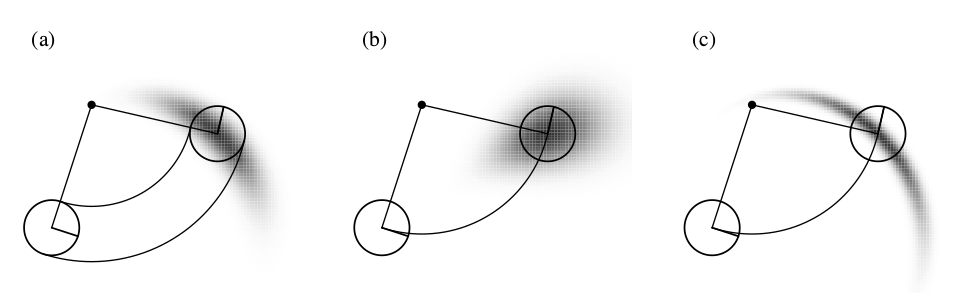
\includegraphics[width=.7\textwidth]{figures/motion_models.png}
	\caption{Velocity motion models for different noise parameters settings. Figure .b shows large translational error and small angular error, Figure .c large angular errors and small translational error}.
	\label{fig:models}
\end{figure}

\subsection{AMCL with GMapping map}

%\textbf{We do not tune the AMLC for both the maps, we keep AMCL params the same as the Graph Localizer and give the two map inputs for comparison (map inputs are the one changing in parameters)}. \\

%The particles of the filter are fixed to \textbf{6000,9000}.

Due to a small deviation (1/2 cm over 37 meters) between the $odometry/filtered$ and the markers, we can assume the EKF to be our ground thruth. We also did some wrong considerations for tuning, please see \textbf{Table5} for the new tuning.

See this link for an answer: https://answers.ros.org/question/227811/tuning-amcls-diff-corrected-and-omni-corrected-odom-models/

\begin{center}
\captionof{table}{alfa parameters and results}
\begin{tabular}{| m{12em} | m{13em}|} 
\hline
\textbf{Parameters} & \textbf{Results} \\
\hline
 alfa4=0.05 &  Just changing this alone did not produce considerable results at all\\
\hline
 alfa4=0.05, alfa3=0.05 &  Also this combinations does not have an effect on the bearing error. The alfas here have been changed to a factor of 20.\\
\hline
 alfa3,4=default=2, alfa1,2=0.05 & Also no result in here \\
\hline
all alfas to 0.1 & Also did not see nothing relevant\\
\hline
alfa1=0.005, alfa2=0.005, alfa3=0.010, alfa4=0.005& No satisfactory results\\
\hline
alfas=0.0001 & works now, I loose global localization property with such a small values, if calling the global localization service. \\
\hline
\end{tabular}
\end{center}

\begin{center}
\captionof{table}{Starting from the corrected alfas = 0,0001, higher progressively alfa3, alfa4 till the optimal}
\begin{tabular}{| m{12em} | m{13em}|} 
\hline
\textbf{Parameters} & \textbf{Results} \\
\hline
alfa3,4=0,001 (try a factor of 10 higher) & Still get considerably good results \\
\hline
\hline
alfa3,4=0,01 (try a factor of 10 higher) & With those value the error is not anymore bounded to the 5 centimeters, hence we keep as a good result the value of before with alfas3,4=0,001. \\
\hline
minparticle = 6000, maxparticle= 9000 & The tuned ones\\
\hline
\end{tabular}
\end{center}

For the update of min{\_} and min{\_}d see the folder update{\_}min{\_}a{\_}d under bagfiles/amcl{\_}localization.

\begin{center}
\captionof{table}{Update min a/d}
\begin{tabular}{| m{12em} | m{13em}|} 
\hline
\textbf{Parameters} & \textbf{Results} \\
\hline
Keep min{\_}d 0.2 and min{\_}a = 0.25 as default values & Plot the difference in changing their values. \\
\hline
\end{tabular}
\end{center}

\begin{center}
\captionof{table}{Final tuning Amcl}
\begin{tabular}{| m{12em} | m{13em}|} 
\hline
\textbf{Parameters} & \textbf{Results} \\
\hline
min{\_}particles= 10 max{\_}particles= 9000 & min is the end number of particles after filter update, max is the spread number at the beginning\\
\hline
min=10, max=9000, alfas=0.2 (default) & Here I am expecting the large error value, infact. \textbf{This works} \\
\hline
Curious to see how the error changes with an max= 12000 & Interesting, with too high particles unable to get convergence, but multimodal distribution. This can be explained by: http://roboticsknowledgebase.com/wiki/state-estimation/adaptive-monte-carlo-localization/. Infact, as the robot moves forward we apply the odom to all the samples (particles), a weight needs to be adressed to all particle, and more resampling steps are needed for convergence. This cause a delay in the filter convergence. \\
\hline
maxparticle 10000 & Converging wrongly\\
\hline
max particle= 9000, alfas.1 & No difference with previous case\\
\hline
mapart= 9000, alfa1,2,3=0.1, alfa4=0.005 (error is translation due to rotation)& No results\\
\hline
maxpart = 9000, alfa1,2=0.1 alfa3,4=0.005 & Converges correctly but no final result\\
\hline
max part = 9000 alfa1,2 = 0.005, alfa3,4=0.1 & Results in wrong convergence after global localization, lost global loc \\
\hline
max part = 9000, alfa1,2 = 0.1,  alfa3,4 = 0.0005 & Still 20 cm error \\
\hline
max part = 9000, alfa1,2 = 0.1,  alfa3,4 = 0.0001 & Still 20 cm error \\
\hline
alfa1,2,3 = 0.1 alfa 4= 0.0001 & If this does not work I keep alfas 3,4 low = 0.0005 and go back with alfa 1,2 till I loose global loc. This does not work\\
\hline
alfa1,2 = 0.08, alfa3,4 = 0.0005 (get alfas 1,2 to a lower value progressively) & No result in lowering progressively alfas 1,2\\ 
\hline
alfa 1,2 = 0.1 and alfa3,4 = 0.00005 & No change\\
\hline
Tried stupid values like 1 & The error is not alfa sensitive \\
\hline
\end{tabular}
\end{center}


%\section{Comparing AMCL with the two different map inputs}



%\section{Comparing Graph-Localizer with the two different map inputs}

%The Graph Localizer is not working with the same params as the AMCL, it should be tuned the same way as the AMCL, starting from particles, then alfas and finally update translation and rotation. We tune this on the \textbf{GMapping tuned} map. 

\end{document}


% == TABLE ==
%begin{table}[h!]
 % \centering
  %\caption{Caption for the table.}
 % \label{tab:table1}
 % \begin{tabular}{ccc}
 %   \toprule
  %  Some & actual & content\\
   % \midrule
   % prettifies & the & content\\
   % as & well & as\\
  %  using & the & booktabs package\\
  %   \bottomrule
  %\end{tabular}
%\end{table}


% === ALGORITHM == 

{\_}

\iffalse % multi-comment tool
\begin{algorithm}[!h]
   \caption{Kirsch, Rohig algorithm}
    \begin{algorithmic}[1]
    	\State $St-1 = St$
        \For{$i = 1$ to $N$} \Comment{With N the number of particles in the filter set by maxparticle parameter}
            \State $Spread $ $particles$ $in$ $the$ $anchorbox$ $with$ $equations$ $1)$ $and$ $2)$ $of$ $[3]$ \Comment{This step is called $Global$ $Localization$}
            
            \State $xt[n] = p(xt|xt-1,ut)$ \Comment{Motion update - sample the particles from the motion update of the robot and move forward to estimate the error model functions}
            
        	\State $wt[n] = p(dnanoLOC|si)*p(dlaser|si)$ \Comment{Measurement update - si are the particles set with i the i-th index}
        	\State $St = St + <xt,wt>$ \Comment{add the state and weight to the total state space}
        	
        	\State $Perform$ $resampling$
        \EndFor
    \State $Return$ $St$

\end{algorithmic}
\end{algorithm}
\fi


\iffalse

\begin{figure}[!htb]
    \centering
    \begin{minipage}{.5\textwidth}
        \centering
        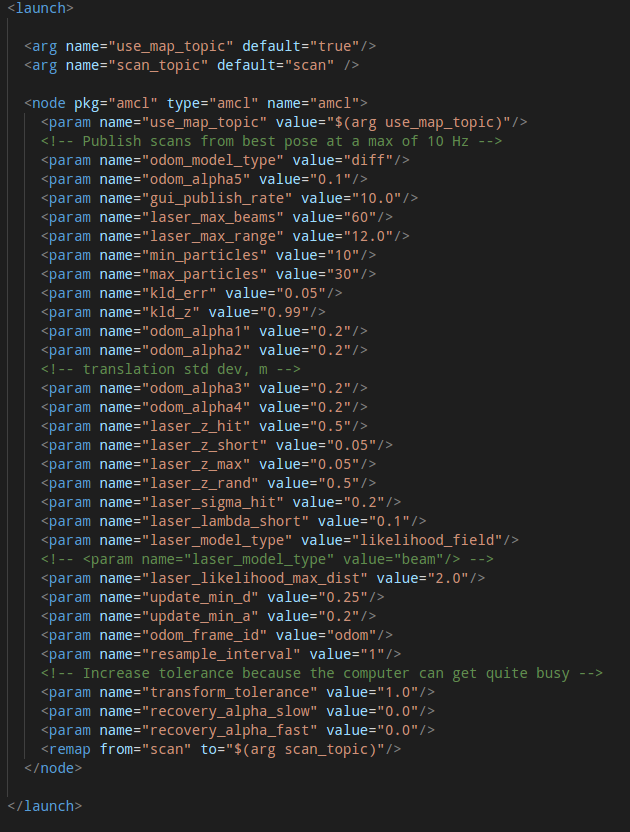
\includegraphics[width=0.7\linewidth, height=0.2\textheight]{figures/amcl_param}
        \caption{The $amcl$ tunable parameters}
        \label{fig:amcl_param}
    \end{minipage}%
    \begin{minipage}{0.5\textwidth}
        \centering
        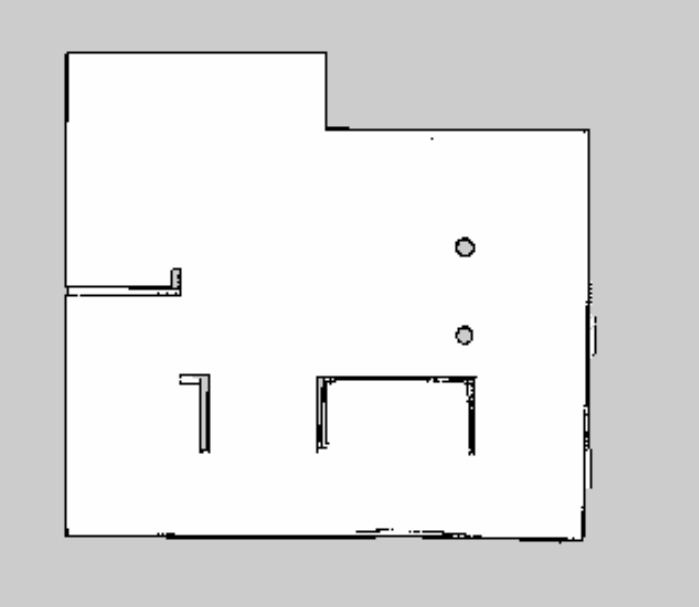
\includegraphics[width=0.7\linewidth, height=0.2\textheight]{figures/my_amcl_gmapping}
        \caption{Result of the Gmapping for the simple indoor environment}
        \label{fig:myamcl_map}
    \end{minipage}
 \end{figure}
 
 
 
\begin{figure}[!htb]
	\center
	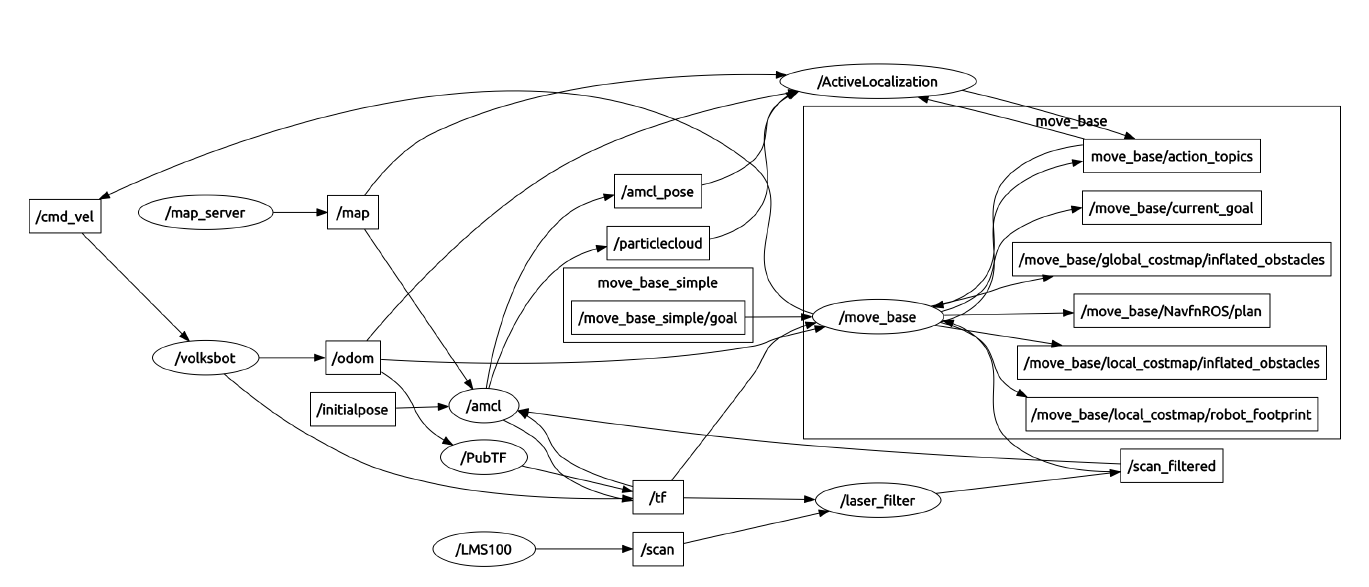
\includegraphics[width=1\textwidth]{figures/active_localization_node.png}
	\caption{An example of an active localization node}
	\label{fig:active_locnode}
\end{figure}


% underscore symbol {\_}

\begin{center}
\captionof{table}{}
\begin{tabular}{| m{12em} | m{13em}| m{12em}|} 
\hline
& &  \\
\hline
\end{tabular}
\end{center}

\fi